\documentclass[letterpaper,11pt]{article}
\usepackage[margin=2cm]{geometry}

\usepackage{graphicx}

\title{\textbf{Pose Fusion with Chain Pose Graphs for Automated Driving}}
\author{HMW-Alexander}

\begin{document}
	
\maketitle

\tableofcontents

\begin{center}\rule{\textwidth}{1pt}\end{center}
\section{Basic Information}

\subsection{Authors}

\begin{itemize}
	\item \textbf{Christian Merfels} is with Volkswagen Group Research, Wolfsburg, and Institute of Geodesy and Geoinformation, University of Bonn, Germany.
	\item \textbf{Cyrill Stachniss} is with Institute of Geodesy and Geoinformation, University of Bonn, Germany.
\end{itemize}

\subsection{Conference}

2016 IEEE/RSJ International Conference on Intelligent Robots and Systems (IROS)

\subsection{Abstract}

\begin{itemize}
	\item Combining multiple localization systems in a \textbf{plug and play manner}.
	\item Formulate this approach as a \textbf{sliding window pose graph}.
	\item The pose fusion approach scales from a filtering-based to a batch solution by increasing the size of the sliding window.
	\item The experiment runs at 20Hz on both simulated and real data.
\end{itemize}

\subsection{Keywords}

\begin{center}\rule{\textwidth}{1pt}\end{center}
\section{Introduction}

\subsection{Problem \& Solution}

Individual localization system is not enough, and the combination of orthogonal localization systems is more powerful.

\subsection{Objective}

This paper provides an approach to multi-sensor data fusion decouples the localization from the fusion task, which eneables the ability to incorporate third-party localization modules for which source code is unavailable.

\subsection{Formulation}

A coarse localization (red triangles), a precise but only temporary available localization (blue triangles), and odometry as dead reckoning trajectory (blue) are used to estimate the true trajectory (red) of a vehicle. The estimated poses are shown as black triangles: the goal is to approximate the unknown red line as closely as possible with the black triangles.

\begin{figure}[!ht]
	\centering
	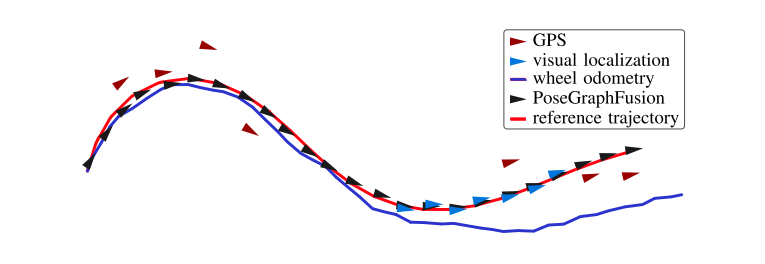
\includegraphics[width=0.8\textwidth]{./img/posefusion.png}
\end{figure}

\subsection{Contributions}

\begin{itemize}
	\item efficient sensor fusion of generic odometry and global pose inputs \(\Rightarrow\) an intuitive architecture for pose estimation and timing issues.
	\item graph construction algorithm \(\Rightarrow\) a sparse block-tridiagonal structure of the system matrix \(\Rightarrow\) fast solution
\end{itemize}

\begin{center}\rule{\textwidth}{1pt}\end{center}
\section{Related Work}

\subsection{Multi-sensor data fusion for navigation systems}

\begin{itemize}
	\item \textbf{filtering-based approaches}: Kalman filter and its variants
	\begin{itemize}
		\item feature: rely at a very early stage on the Markov assumption and marginalize all older information
		\item problem: prematurely incorporating the linearization error.
	\end{itemize}
	\item \textbf{sliding window smoothing algorithms}: compute the maximum likelihood (ML) estimate by nonlinear least squares optimization to a Bayesian network, Markov random field (MRF), or factor graph.
	\begin{itemize}
		\item feature: consider all past measurements up to the current one; and also consider future measurements for offline batch optimization.
		\item solution: online batch optimization becomes feasible through the usage of incremental smoothing techniques, such as iSAM2\footnote{M. Kaess, H. Johannsson, R. Roberts, V. Ila, J. Leonard, and F. Del- laert, “iSAM2: Incremental Smoothing and Mapping using the Bayes tree,” Int. Journal of Robotics Research, pp. 216–235, 2012.}, that recalculate only the part of the graph that is affected by new measurements.
		\item Some implementations keep the size of the graph bounded by simply discarding older nodes and edges, thus potentially obtaining overconfident estimates.
	\end{itemize}
\end{itemize}

\subsection{Methodical origin}

\begin{itemize}
	\item Sibley et al.\footnote{G. Sibley, L. Matthies, and G. Sukhatme, “SlidingWindow Filter with Application to Planetary Landing,” Journal of Field Robotics, vol. 27, no. 5, pp. 587–608, 2010}, who are the first to introduce the concept of a slibing window filter in the context of robotics.
	\item Differences:
	\begin{itemize}
		\item apply this to the use case of pose fusion
		\item special design for a faster way of solving the nonlinear least squares equations, performing marginalization, and estimating the uncertainty of the output.
		\item provide a way of semantically reasoning about the prior information arising from marginalization by deriving a prior node.
	\end{itemize}
\end{itemize}

\section{Pose Graph Fusion}

\subsection{Nonlinear least squares problem}

This paper exploits the state-of-the-art graph optimization framework g2o\footnote{R. K¨ ummerle, G. Grisetti, H. Strasdat, K. Konolige, and W. Burgard, “g2o: A General Framework for Graph Optimization,” in Proc. IEEE Int. Conf. Robotics and Automation (ICRA), 2011, pp. 3607–3613.}.

The key idea is that given the state vector \(x=(x_1^T, ..., x_m^T)^T\) and a set of measurements, where \(z_{ij}\) is the mean and \(\Omega_{ij}\) is the information matrix of a single measurement relating \(x_i\) to \(x_j\), least squares estimation seeks the state
\[x^*=\arg\min_x{\sum_{i,j}e_{ij}^T\Omega_{ij}e_{ij}}~~~~(1)\]
that best explains all measurements given the \(\mathcal{l}_2\) norm. The vector error function \(e_{ij}=e(x_i,x_j,z_{ij})\) measures how well the constraint from the measurement \(z_{ij}\) is satisfied. Solving (1) requires iteratively solving a linear system with the system matrix \(H\) and the right-hand side vector \(b\) such that
\[H=\sum_{i,j}{J_{ij}(x)^T\Omega_{ij}J_{ij}(x)}\]
\[b^T=\sum_{i,j}e_{ij}^T\Omega_{ij}J_{ij}(x)\]
where \(J_{ij}(x)\) refers to the Jacobian of the error function computed in state \(x\).

\subsection{Sliding window chain pose graph fusion}

\subsubsection{About the online state estimation system}

\begin{itemize}
	\item general nonlinear least squares estimation taks into account all available information within the full pose graph
	\item to keep the problem computationally tractable, it is necessary to limit the considered information.
	\item this approach achieves this by marginalizing out prior state state variables and the state vector \(x\) in a sliding window pose graph is reduced to the M most recent states \(x=(x_{t-M+1}^T,...,x_t^T)^T\).
\end{itemize}

\subsubsection{About the graph structure}

\begin{itemize}
	\item global pose source: measure poses within a global coordinate system, e.g. Universal Transverse Mercator (UTM) coordinate
	\item local pose source:  measure spatial transformations relative to the previous pose, e.g. odometry
	\item hidden nodes (from MRFs): state variables
	\item observed nodes (from MRFs): global pose constraints, connected to hidden nodes to constrain them in the global coordinate frame.
	\item edge between hidden nodes: local pose constraints.
	\item The resulting form or the graph is called \textbf{chain pose graph}.
\end{itemize}

\begin{figure}[!ht]
	\centering
	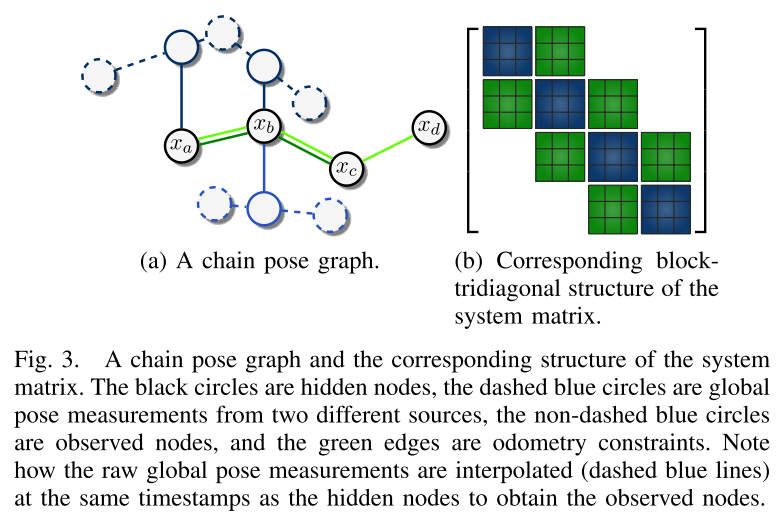
\includegraphics[width=0.8\textwidth]{./img/posegraph.png}
\end{figure}

\subsubsection{About the algorithm working frequency}

\begin{itemize}
	\item Related graph-based approaches.
	\begin{itemize}
		\item generate a hidden node (state variables) every time a measurement arrives
		\item or tie their generation to a specific pose source
	\end{itemize}
	\item This approach constructs a hidden node every time stamp.
	\begin{itemize}
		\item it queries all global pose sources for measurements and interpolate one observed node per source at the timestamp of the hidden node if measurements are available.
		\item it queries each local pose source to interpolate the edges between all two successive hidden nodes.
		\item enforce a certain matrix structure for H, to include all measurement sources in a generic way independetly of their specific output frequencies, and to a priori relate the number of state variables to the length of the interval of the sliding window.
	\end{itemize}
\end{itemize}

\subsubsection{About the system matrix}

\begin{itemize}
	\item The block-tridiagonal 
\end{itemize}

\end{document}